%!TEX root = ../thesis.tex
\chapter{Introduction}\label{chap:Introduction}

% Justify studying emotions
Why is it important to study emotion?
Emotions are considered a human state that influences behaviour and decision making. Many times, when expressing thoughts in a written or spoken form, one or several emotions are present. Detecting these emotions is an important task for human interaction. Automatic emotion detection on text is thus a machine learning task required for comprehensive human-computer interaction.

\section{Emotions and Affect}\label{sec:Emotions and Affect}

In the endless effort towards understanding human behaviour the phenomenon of Emotions has been recognized for centuries. It is after all, an experience that every human has. For many of us it represents a core variable in the representation of our biological, psychological, and social state. For such an important part of our lives, it is incredible how little we actually know about them. There is no scientific consensus on what an emotion is, and the term is often used to refer to mood, humor, temperament, personality, affect, character, and sentiment.
This section has as a goal to point out relevant discoveries and conceptualizations in the history of the study of emotions, as a way of delimiting the current study, and as a mean of introduction to the topic for technology-focused readers, but also as a way of outlining a working definition of Emotion, differenciating it from Affect.

\subsection{Historic Milestones}\label{sub:Historic Milestones}

% Hippocrates and Galen
Hippocrates, the father of modern medicine, defined the theory of the Four Humors.
This was based on the idea of humors, fluids, or chemicals that control human behaviour.
The four humors should be in balance within the body, and all diseases were caused by an inbalance of these.\cite{kalachanis2015hippocratic}
Galen at took this theory and created what can be considered as the first theory of personality. He believed that human bodies had a predisposition for unbalance of the humors. This made some people have a tendency to have more or less of these, and in turn, this would have an effect on their baseline behaviour. He described four different characteristical behaviours: phlegmatic, choleric, sanguine and melancholic.\cite{irwin1947galen}

\begin{figure}[H]
  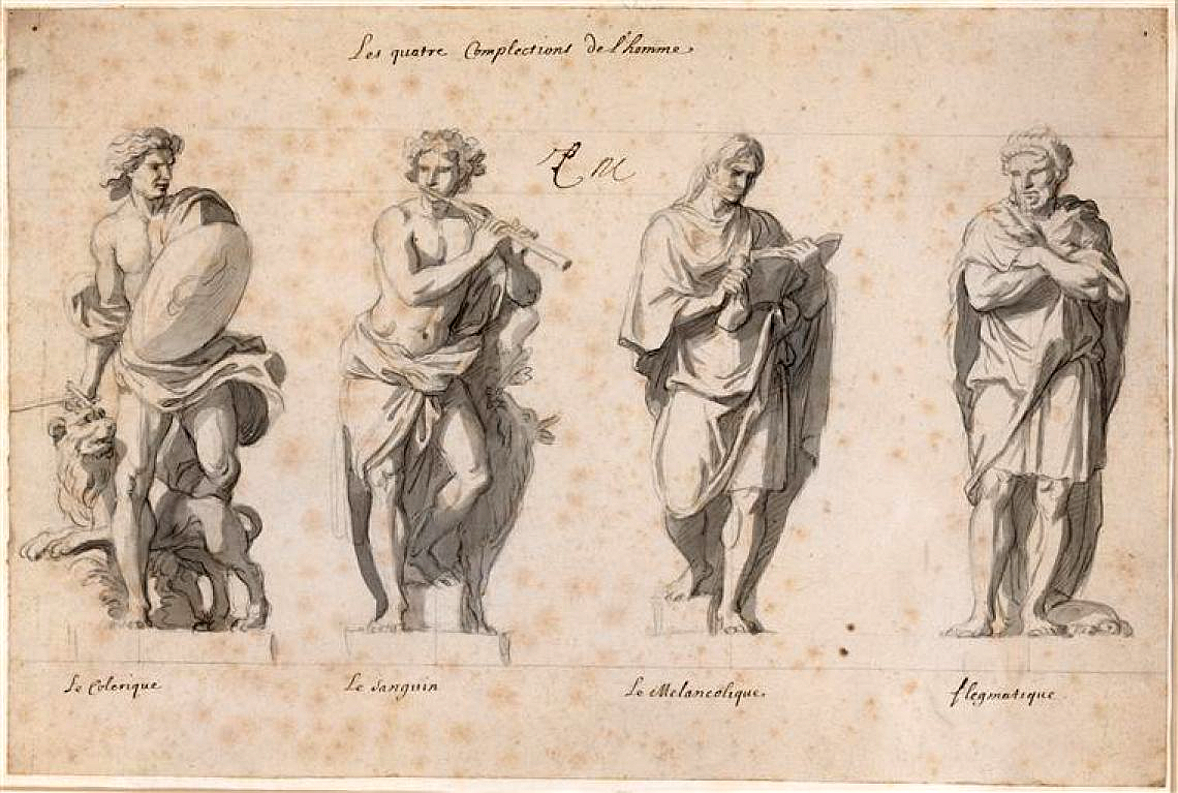
\includegraphics[width=1\textwidth]{temperaments}
  \centering
  \caption{Wikicommons PD. The four temperaments by Charles Le Brun, part of the \emph{Grande Commande}.}
\end{figure}\label{fig:temperaments}

% Darwin
Charles Darwin first described the importance of emotions in communication, and their relevance across cultures and even species. In his book ' \emph{The Expression of the Emotions in Man and Animals} ' he writes ' \ldots the young and the old of widely different races, both with man and animals, express the same state of mind by the same movements.' ~\cite{darwin1872emotions} He noticed that surprise was shown in humans across cultures, and even some mamals by raising the eyebrows. By framing emotions as a mean of communication, Darwin enabled the study of expression, and understanding of emotions as an evolutive advantage.

\begin{figure}[H]
  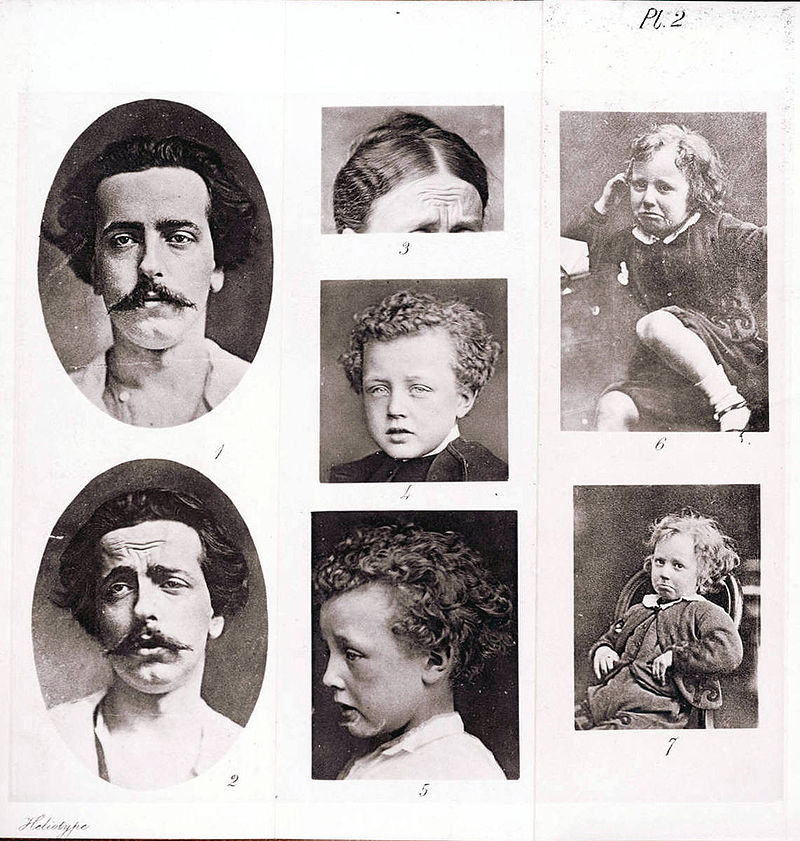
\includegraphics[width=1\textwidth]{darwin}
  \centering
  \caption{Wikicommons PD. Ilustration of grief from Darwin's \emph{"The Expression of the Emotions in Man and Animals"}}
\end{figure}\label{fig:darwin}

% Ekman
Although Emotions were thought to be universal there was no measurement of it. The universality of emotions was first formalized by Paul Ekman in his 1997 paper: "Universal facial expressions of emotion". Ekman studied facial anatomy, and expressions of different populations and cultures across the globe. He arrived to the conclussion that there are seven universal facial expressions of emotion~\cite{ekman1997universal}.

\begin{figure}[H]
  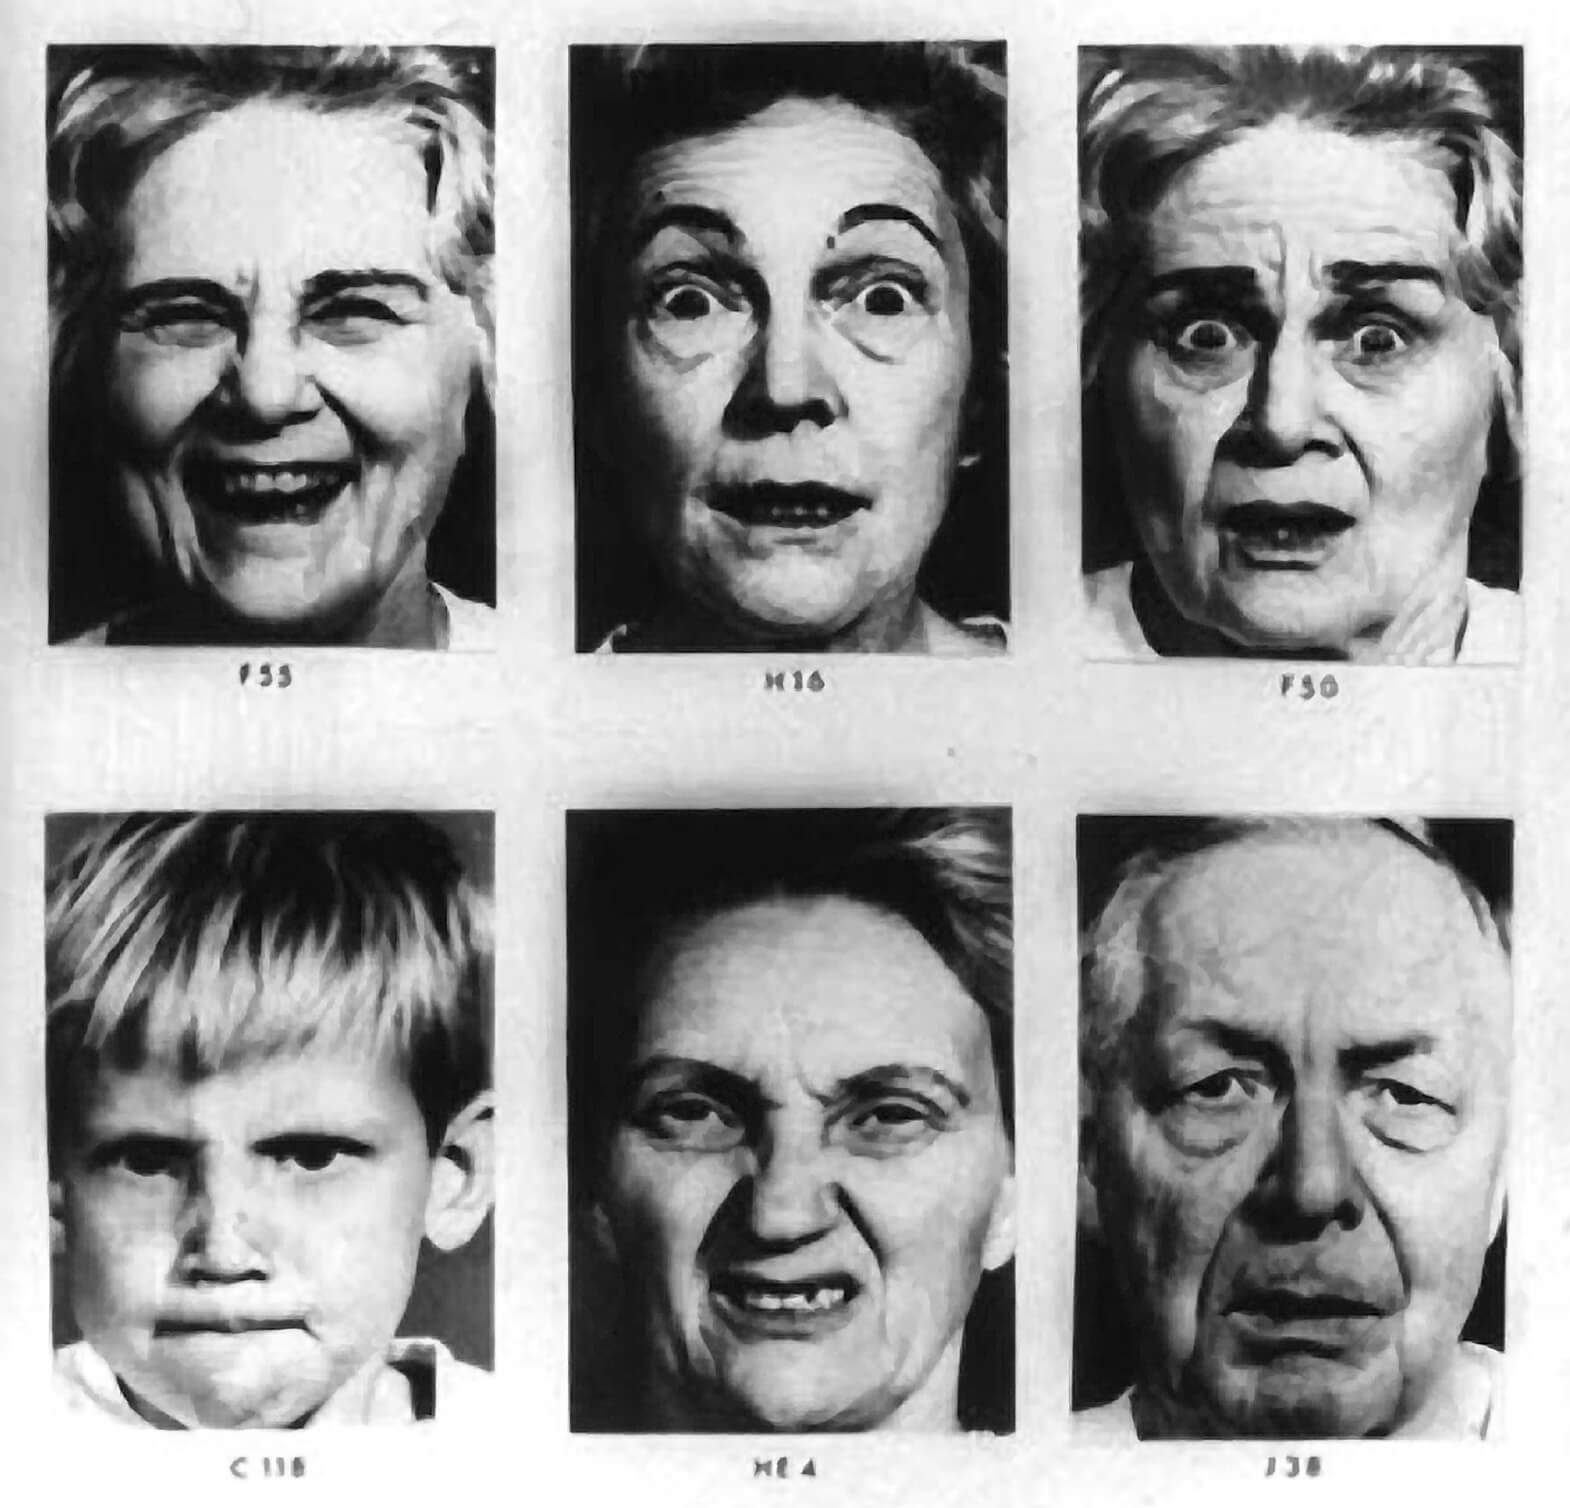
\includegraphics[width=1\textwidth]{ekman}
  \centering
  \caption{Ekman's photographs for cross-cultural research~\cite{ekman1999facial}.}
\end{figure}\label{fig:darwin}

% Picard
While emotions are a human concept, the digital advances of thte milenium caught up and integrated with the field, to create the Affective Computing. The concept was first coined by Rosalind Picard, who not only created it, but is also a lead researcher in the field~\cite{picard2000affective}. The concept was originaly related to Human-Computer interactions, and had the goal of computers expressing and recognizing emotions.

% Plutchik
Concerned with the subjectivity of emotion messurement, and the lack of generalization of self-report affect scales, Robert Plutchik proposed a method of meassuring the baseic emotions in a systematic way. He also proposed a way of derivating new emotions from the universal set proposed by Ekman. This was to be done based on theory, with enough diversity, but systematically relatable to the universal emotions~\cite{plutchik2013measurement}. In this way, the Plutchik model of emotions was created. This model is based on Ekman's universal emotions. Today, most Machine Learning tasks and datasets use this model of emotions. Different models will be discussed further in this chapter.

% Feldman
It is important to consider that for the last two decades, emotions have been studied based on Ekman's work on universal emotions. Although these do provide a framework for understanding how emotions came to be a part of the human experience, they do very little for their definition, or the description of emotions in language. Humans are complex, and even the most reliable model of universal emotions has exceptions. Psychologists interpret those differences with the help of the Theory of Constructed Emotions. This was first published by Lisa Feldman in 2014, and it describes the phenomenon of human emotions as a two-sided event: Affect and Emotion. Affect is a physiological phenomenon, the almost mechanical process that will enable behavioural response. The Emotional response is the cognitive contextualization of the former~\cite{feldman2014constructed}. Separation of physiological and cognitive responses allows the explanation of both, universality, and individual subjectivity.


% Woring Definition of emotion
\subsection{Definition of Emotion}\label{sub:Definition of Emotion}
Within the context of this project it is important to distinguish between emotion and affect. Affect, in the context of this project will be treated as a term to associate predisposition towards stimuli. Thus, affect is in a sense, a general term that can be even used to describe animal, and other non-human entities. Emotions, on the other hand, are treated in this project as a state inherent to humans. This state is multidimensional, and every dimension, or emotion, can either be present in a certain amount, or not be present at all.
Emotions present an affect value, but not necessarily otherwise.


% DELIMITATION

\subsection{Affect}\label{sub:Affect}
In the context of this project the term Affect will be used to denote the autonomus physiological response of the human body to external stimuli, as well as the measure of these in terms of Valence, or Arousal. This definition complies with the Theory of Constructed Emotions, whithout invalidating the extended use of affect models of language.

The relevance of affect in text has increased since the popularization of text-based social networks, like twitter. There, individuals and organizations openly express their opinions. This creates an environment where implicit feedback about entities is present. An easy way to abstract popular opinion about a named entity is learning the affect expressed in text, such as a tweet. Affect can be a multidimensional phenomenon, but the most important dimension of it is valence: whether a text expresses positive or negative emotion. This use of affect language models has proven useful to marketing, public relationship, and social sensing, but does not provide an insight into the human experience of emotion further than a signle dichotomical variable.

Affect is relevant to this project since emotions can be represented within the models of affect that include valence and arousal~\cite{barradas2016thesis}.

\subsection{Emotions in Communication}\label{sub:Emotions in Communication}
The main evolutive advantage of emotions is to be able to communicate an internal state with others. The communication, and therefore, the detection of emotions can be done through three different means:
\begin{itemize}
  \item \textbf{Language or self report}: Using language, verbal, written, or otherwise, to express content with emotion, or explicitly declare an emotional state.
  \item \textbf{Facial Expressions}: The activation of different sets of facial muscles to express emotion. This must be measured visualy.
  \item \textbf{Biosignals}: The change of physiological states usually related to the limbic system can be measured through bio-sensors. This more accurately represent affect, but emotions can be measured through it.
\end{itemize}

This project is focused on language expressions of emotion. More specifically on expressions of emotion through text. This means that this project will not directly measure emotions on humans, but on text written by humans. These represent the expresion of a momentary emotional state, expressed through text, and stored for later analysis. Text analysis is a subset of the field of Natural Language Processing (NLP). This project is heavely based on NLP concetps. For this reason, different methods for emotion analysis in text are discussed next.

\subsection{Models of Emotions}\label{sub:Models of Emotions}
When searching for expressions of emotions in text, one must know what kind of emotions are being searched for. When asking a person what emotions do they know, a plethora of emotions can be named, but most of these are language, culture, or context dependant. Under certain cultures, or even sub-cultures, new emotion names can emerge, that describe a general emotion under different context. Considering the theory of constructed emotions, there is as many emotions as context there are. Fortunately, the study of emotions being done here is restricted to the communication of emotions. For the communication of emotions a consensus must be made.
A model of emotions is the selection and structure of categories in which the expression of an emotion can fall, commonly called 'Universal Emotions'. These are usually formed through the analysis of human (and some times animal) behaviour, with the framework of a theory of behaviour. In this section we introduce some relevant models of emotion for ML and NLP.

\subsubsection{Ekman's model of Emotions}\label{subs:Ekman's model of Emotions}
As mentioned in \ref{sub:Historic Milestones}, the most widely recognized model of universal emotions in humans was created by Paul Ekman\cite{ekman1992basic}. This was created through the observation of facial expressions. Facial expressions are measured through Activation Units (AU's): Sets of muscles that, when contracted, deform the figure of the human face in specific ways. Emotions are then characterized by the activation of different sets of AU's. The current model of universal emotions contains seven emotions:

\begin{itemize}
  \item Anger
  \item Disgust
  \item Fear
  \item Surprise
  \item Happiness
  \item Sadness
  \item Contempt
\end{itemize}

Although this model is based on facial expressions, most studies of emotion use this as the base model to explore and understand concepts of human behaviour. Notice that this model is based on the communication of emotions through facial expressons. These are said to be universal because facial expressions seem to have been forged through natural selection, and are independant of culture, language, or segregation of populations. In simple terms, humanity had a face for longer than most other human traits. Under this frame of reference, language as a mean of communication is a relatively new phenomenon, but since it allows for more detailed communication, it changes the way we communicate our internal states.

\subsubsection{Plutchik's model of Emotions}\label{subs:Plutchik's model of Emotions}
Although Ekman's model provides a firm base for universal emotions, it lacks structure. Robert Plutchik created his model by removing Contempt, and adding two more emotions: anticipation and trust. By doing so, a three-dimentional model was createt that also provided dichotomical, or polar emotions, intensities, and derivatives through superposition.

\begin{figure}[H]
  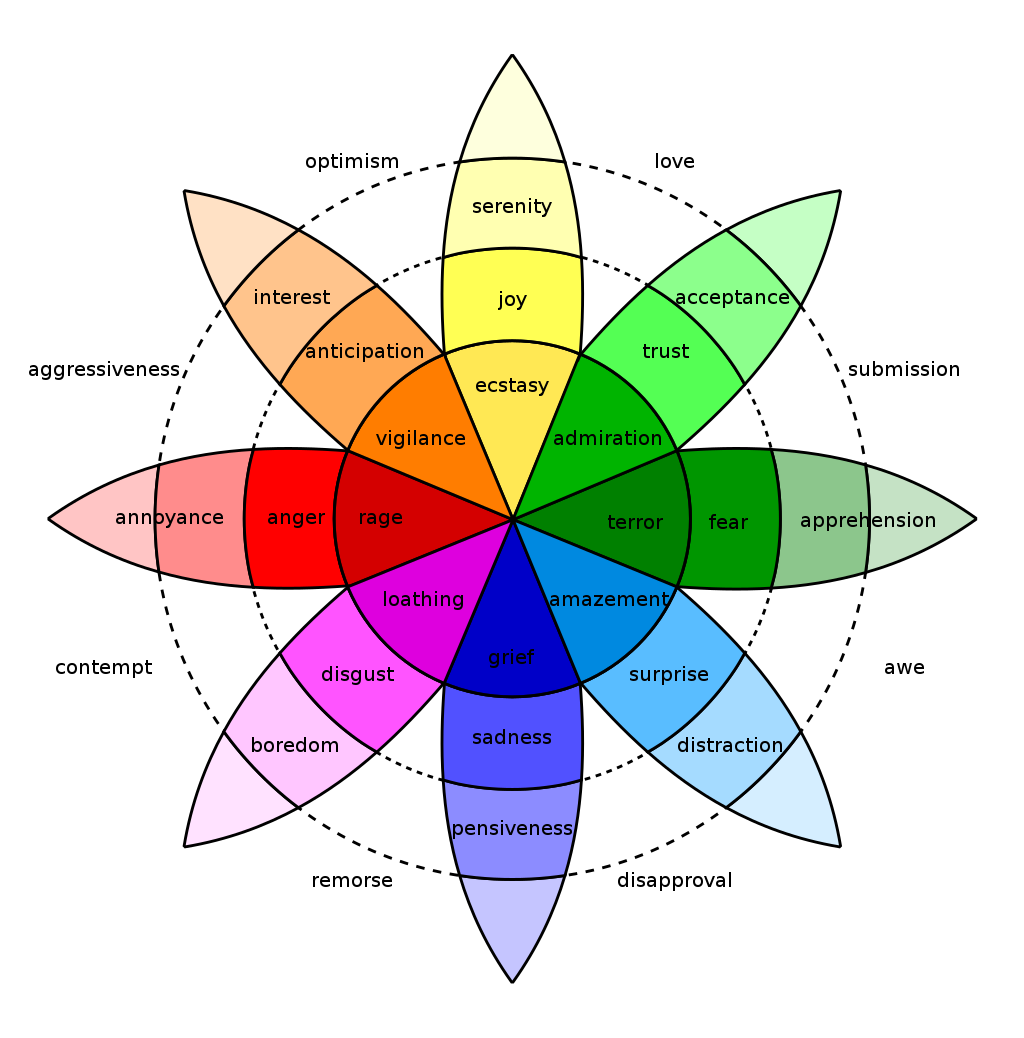
\includegraphics[width=1\textwidth]{plutchik}
  \centering
  \caption{Wikicommons PD. Plutchik's wheel of emotions}
\end{figure}\label{fig:plutchik}

The model shown in figure \ref{fig:plutchik} shows these characteristics. The main emotions are expressed in different intensities, and named acordingly. The combination, or superposition of some emotions receives a new name. This model is so well structured and colored, that it has called the attention of the scientific and engineering community. Unfortunately the premises of this model are faulty, and the scientific basis are questionable. The subjective nature of emotions doesn't allow for strict dichotomies. A simple poll asking 'What's the opposite of joy?' will turn in two answers: Anger and Sadness, deppending on the context.

Acording to the theory of Constructed Emotions, it is exactly context that creates emotions. This means that culture, language, learning, and many other environmental factors contribute to the characterization of an emotion. For this reason, when studying emotions in text, a mean of contextualizing an emotion word is necessary.

\subsection{Emotions and Text}\label{sub:Emotions and Text}
When it comes to contextualizing words, linguists have had tools since the 1930's~\cite{corson1996fields}. This is the case of Lexical Fields. In it's simplest version, this tools ask people what words are most closely related to a concept. The result of a free assosiaton can be a network of interrelated words, or a set of words that relate to a concept. This set is also called a semantic field.
By asking people what emotions are related to a specific word, a semantic field of emotions can be created.

% TODO: text on border
This is exactly what Saif Mohammad did in 2013~\cite{mohammad2013crowdsourcing}, creating the Canadian National Research Counsil Emotional Lexicon (NRC EmoLex). This contains around 14 thousand words, and their association with the 8 basic emotions of the plutchik emotion model. This was an incredible effort, since several people must review every single word and emotion relationship, and evaluate them.
All this work can actually be infered from large corpus. By creating a network of word relationships, WordNet provides a way to cluster into affective words~\cite{strapparava2004wordnet}. This proves that a representation of emotions in text can be learned from text, without human intervention. Machine Learninng provides tools to optimize this representations.

\section{Emotion and Machine Learning}\label{sec:Emotion and Machine Learning}
The field of Natural Language Processing has seen great advances in recent years thanks to the use of Machine Learning for automatic inference of language models.

While there are many ways of using ML within NLP, the methodology this project focuses on is Word and Sentence Embedding. Embedding is the process of giving a numeric representation to a word or sentence within a corpus. This allows for computational models to easily manipulate text data that would otherwise be an arbitrary encoding of text. With the advances in machine learning automatic word embedding became a possible solution to avoid crowdsourcing.

Several machine learning approaches try to automatically learn the best numeric representation for characters, words, or sentences given the context of a dataset. In the last decade there have been many efforts from research groups to generalize these embeddings though the use of powerful models, and bigger datasets.

% Word2Vec
One of the first models to call the community's attention was Google's Word2Vec\cite{mikolov2013word2vec}. A model trained on news articles that allowed for complex languge representation, like lexical artimetic. This model has the model of an Autoencoder, and is therefore unsupervised.
% Should I talk more about dimensionality reduction/ autoencoders?

After Word2Vec, a series of language models were created. Word2Vec sccessors include ELMo, GloVe, which are similar but consider more or different context when creating the language model. With the creation of the transformer in ML~\cite{vaswani2017transformer}, a second wave of ML language models were created. XLM, GPT, BERT and it's many iterations, all provide a language model that captures not only the representation of a word, but also it's context.

These models learn to represent words from context: By looking at the words and sentences in a document, a contextualization is given to the use of a specific word, in every document. These language representations are far from a lexicon. They are numerical representations that, due to their automatically learned creation, are difficult for humans to interpret. Once these models are trained on large amounts of data, the trained model can be stored, and re-distributed to be used in different language tasks. This is called a pre-trained model. For this reason, such a context-dependant model can be used in short sentences, or even single words: The model is in itself the abstraction of a large amount of language data, learned through text documents.
There exist also models trained not on documents, but on dialogues. These models will not be used in the context of this project.

By observing the abstract representations of these models, one can learn how specific concepts are learned by pretrained ML models from text.

\section{Problem setting}\label{sec:Problem setting}

Given pre-trained language models, and corpus of labeled text with single emotions, can we find the similitude between the structure of the representation of said text and their emotions in the abstract space created by the language model and a model of emotions backed up by scientific research?

\section{Objective}\label{sec:Objective}

To quantifiably and objectively analyze the representation of emotions in Machine Learning pre-trained Language Models, while presenting a human-understandable cualitative description to promote the discussion of models of emotions and atuomatic learning of human concepts in Natural Language Processing, and Machine Learning.

As consequence of this objective, the methodology to analyze a dataset of labeled emotions based on pre-trained language models is to be established. The intuitions and qualitative results of this project are to be developed into actual analysis methods to be used in the understanding of language models.


\section{Justification}\label{sec:Justification}
Be it in dialogue, local or international media, or even entretainment, current events have proven that the incorrect understanding of the emotional response of the general population can lead to severe social problems. Subcultures, minorities, and opressed populations are expressing their problems and difficulties in plataforms all around the internet. People need to express themselves,be heard and understood, as well as understand other points of view, but untrained emotional reaction is being weaponized to duscourage discussion, dialogue, and democracy. Be it as a political or military action, or simply by lack of self conciousness, the emotions of every technology user and media consumer can turn against themselves. Justified pacific protests can turn into meaningless riots. Rational arguments can turn into senseless discussions, that separate populations and capture us in our subjective realities. I believe that the understanding, awareness, and acceptance of our emotions and others' can lead towards the path to dialogue, comprehension and peace. To do so at a scale as large as the one presented by the internet, and global media, we must use the same tools that have created such a vast field. The understanding of our data, ML and AI models, and their representations of our reality can help us understand ourselves. This project is at it's core, an atempt at understanding human nature.
